%\section{Projection results}
\paragraph{Model-independent limits}
\label{sec:model_indep}

The model-independent limits on the cross section of the ggH and bbH production mechanisms with subsequent $\tau\tau$ decays are shown in Fig.~\ref{fig:model_indep} for 
integrated luminosities of 300\fbinv and 3000\fbinv.
For both production modes, the improvement at high mass is close to the statistical limit of scaling with the square root of the integrated luminosity, 
see Fig.~\ref{fig:model_indep2}. 
The improvement at very low mass is almost entirely due to the assumption of reduced systematic uncertainties, and not directly due to 
the additional collected data in the signal region. The difference between the Run 2 and YR18 scenarios is mostly due to the treatment 
of two kinds of systematic uncertainties of statistical nature, namely the uncertainties due to the number of simulated events and the number 
of events in data control regions.
%
\begin{figure}[htbp]
\begin{center}
\subfloat[ggH]{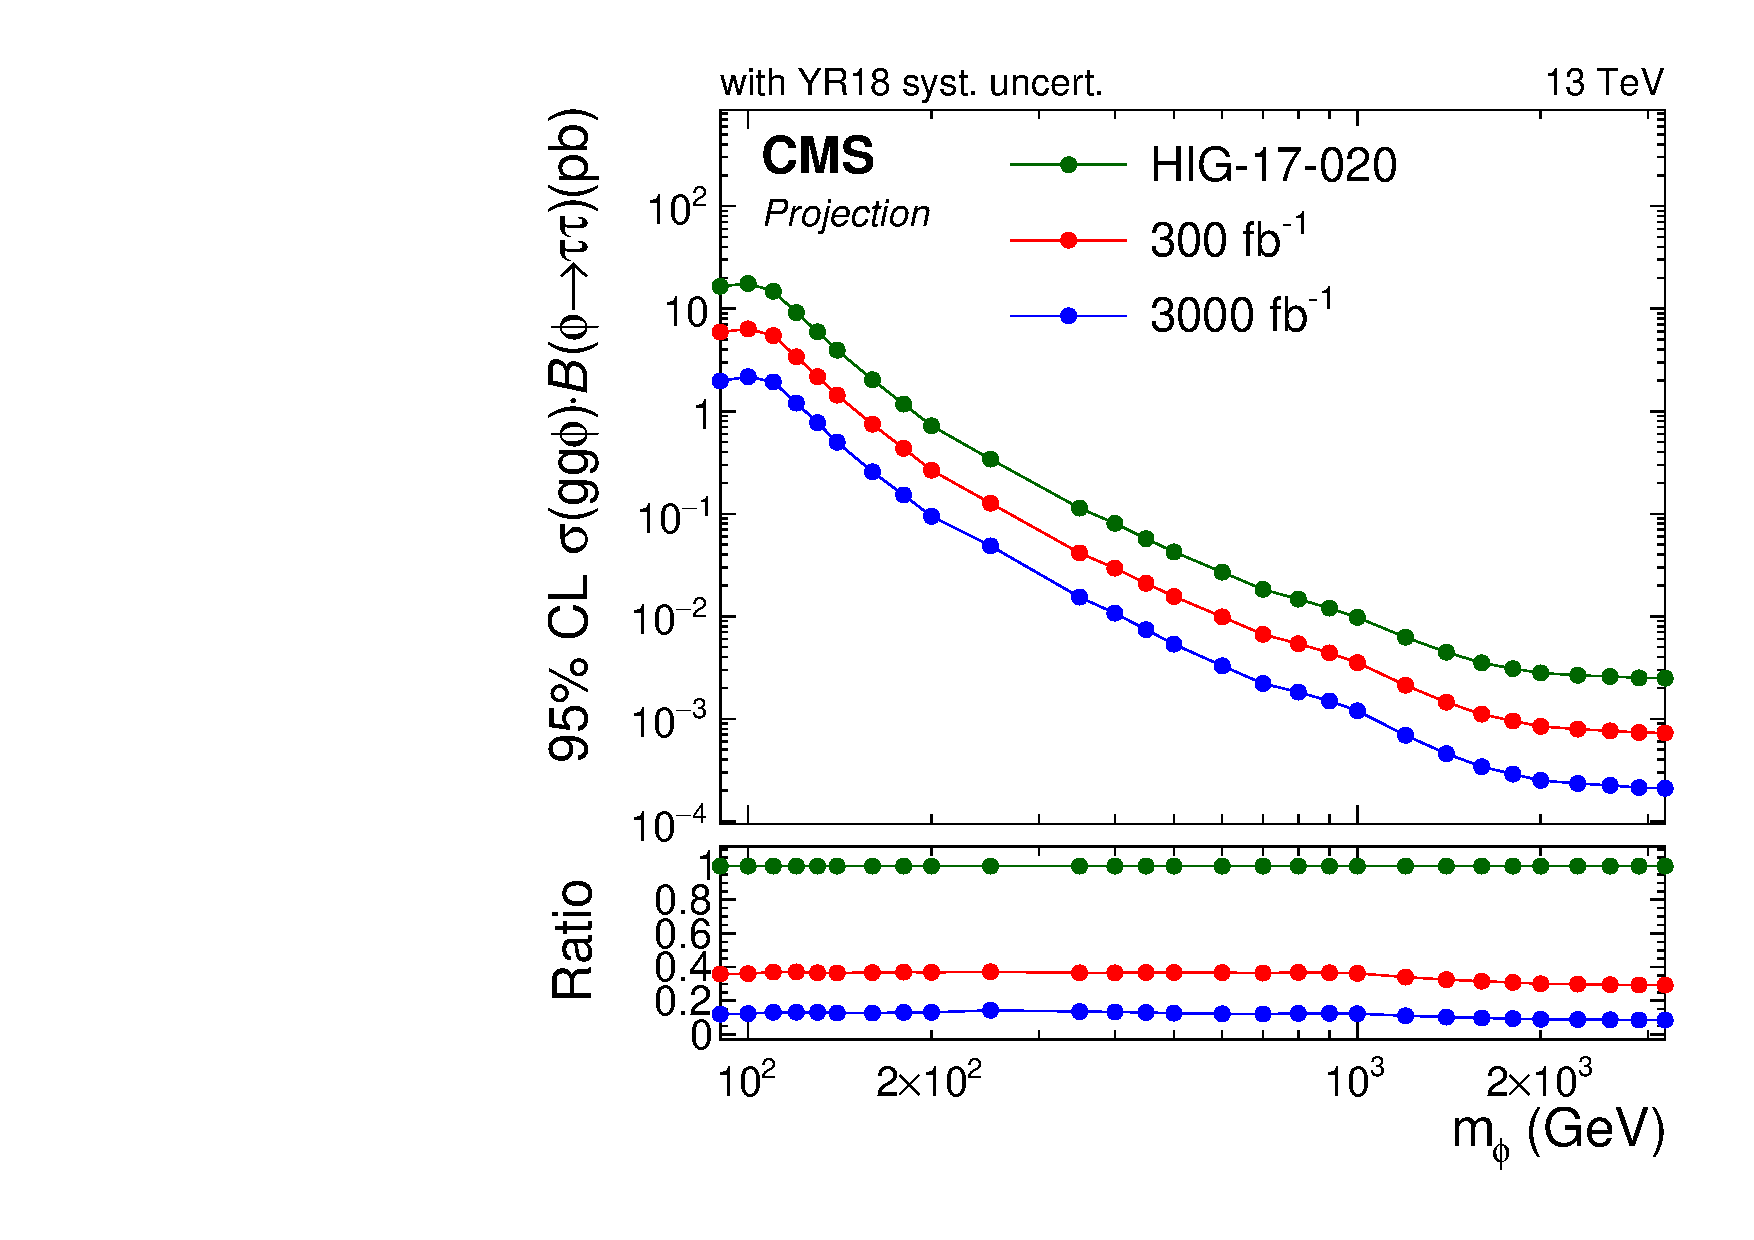
\includegraphics[width=0.45\textwidth]{\main/section9/plots/scen2_ggH_pas.pdf}}
\subfloat[bbH]{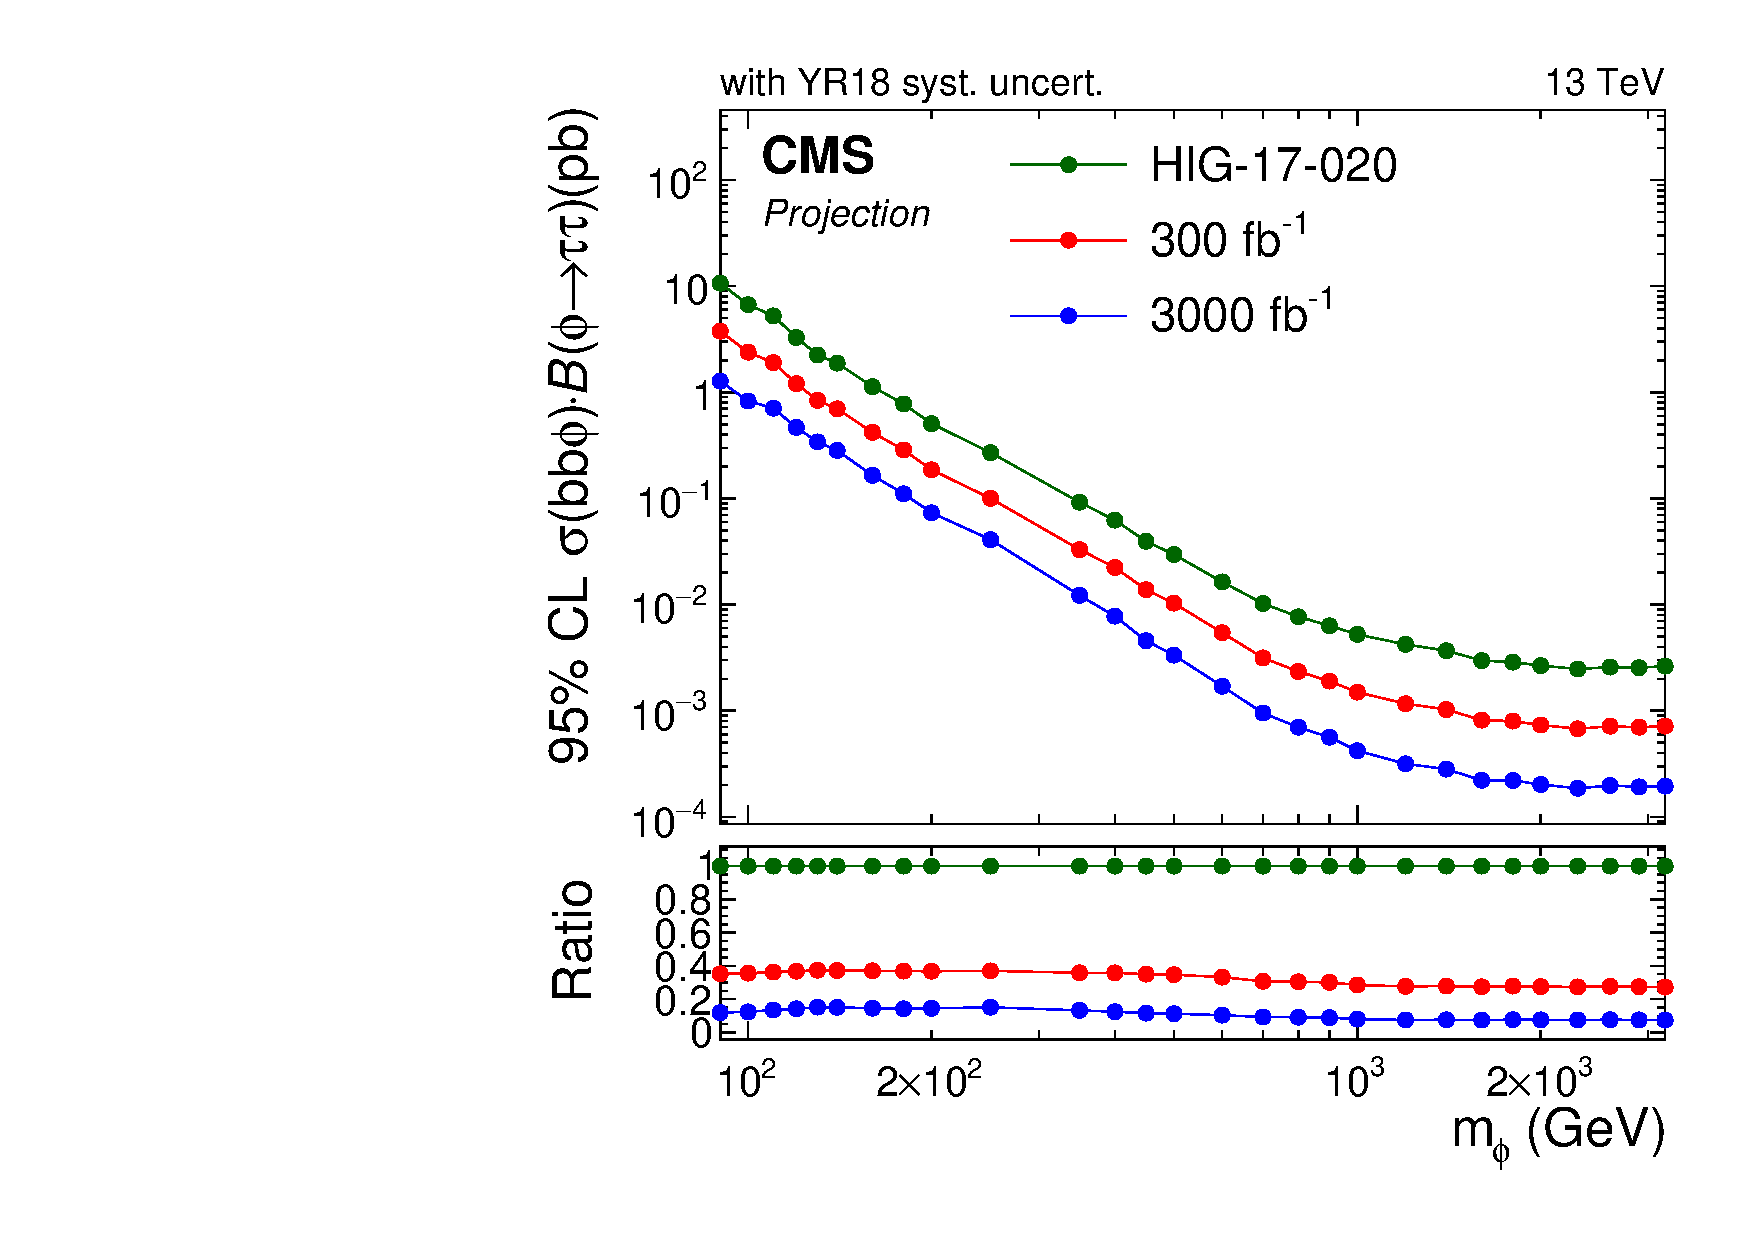
\includegraphics[width=0.45\textwidth]{\main/section9/plots/scen2_bbH_pas.pdf}}
\end{center}
\caption{Projection of expected model-independent limits based on 2016 data~\cite{HIG-17-020} for ggH and bbH production with subsequent \htt decays, with YR18 systematic uncertainties.}
\label{fig:model_indep}
\end{figure}
%
\begin{figure}[htbp]
\begin{center}
\subfloat[ggH]{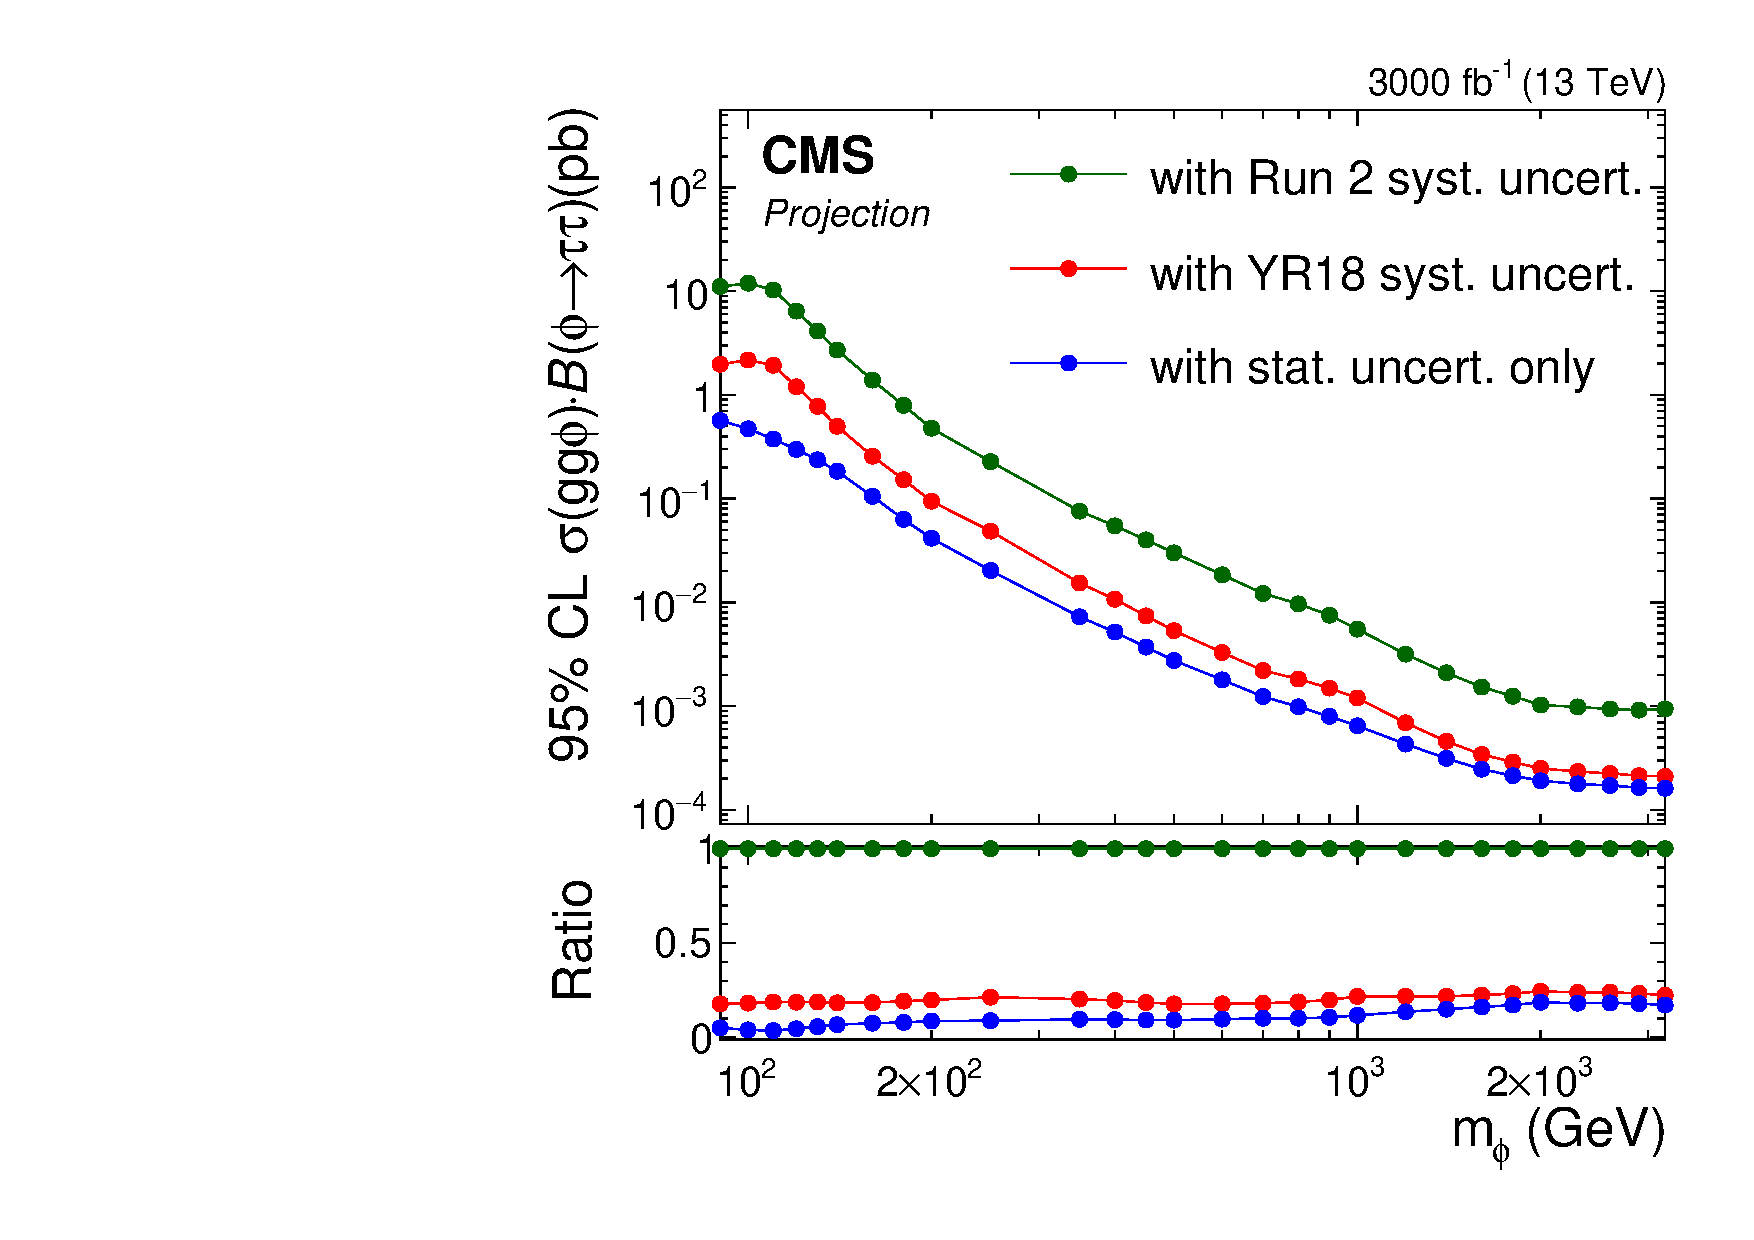
\includegraphics[width=0.45\textwidth]{\main/section9/plots/3000fb_ggH_pas.pdf}}
\subfloat[bbH]{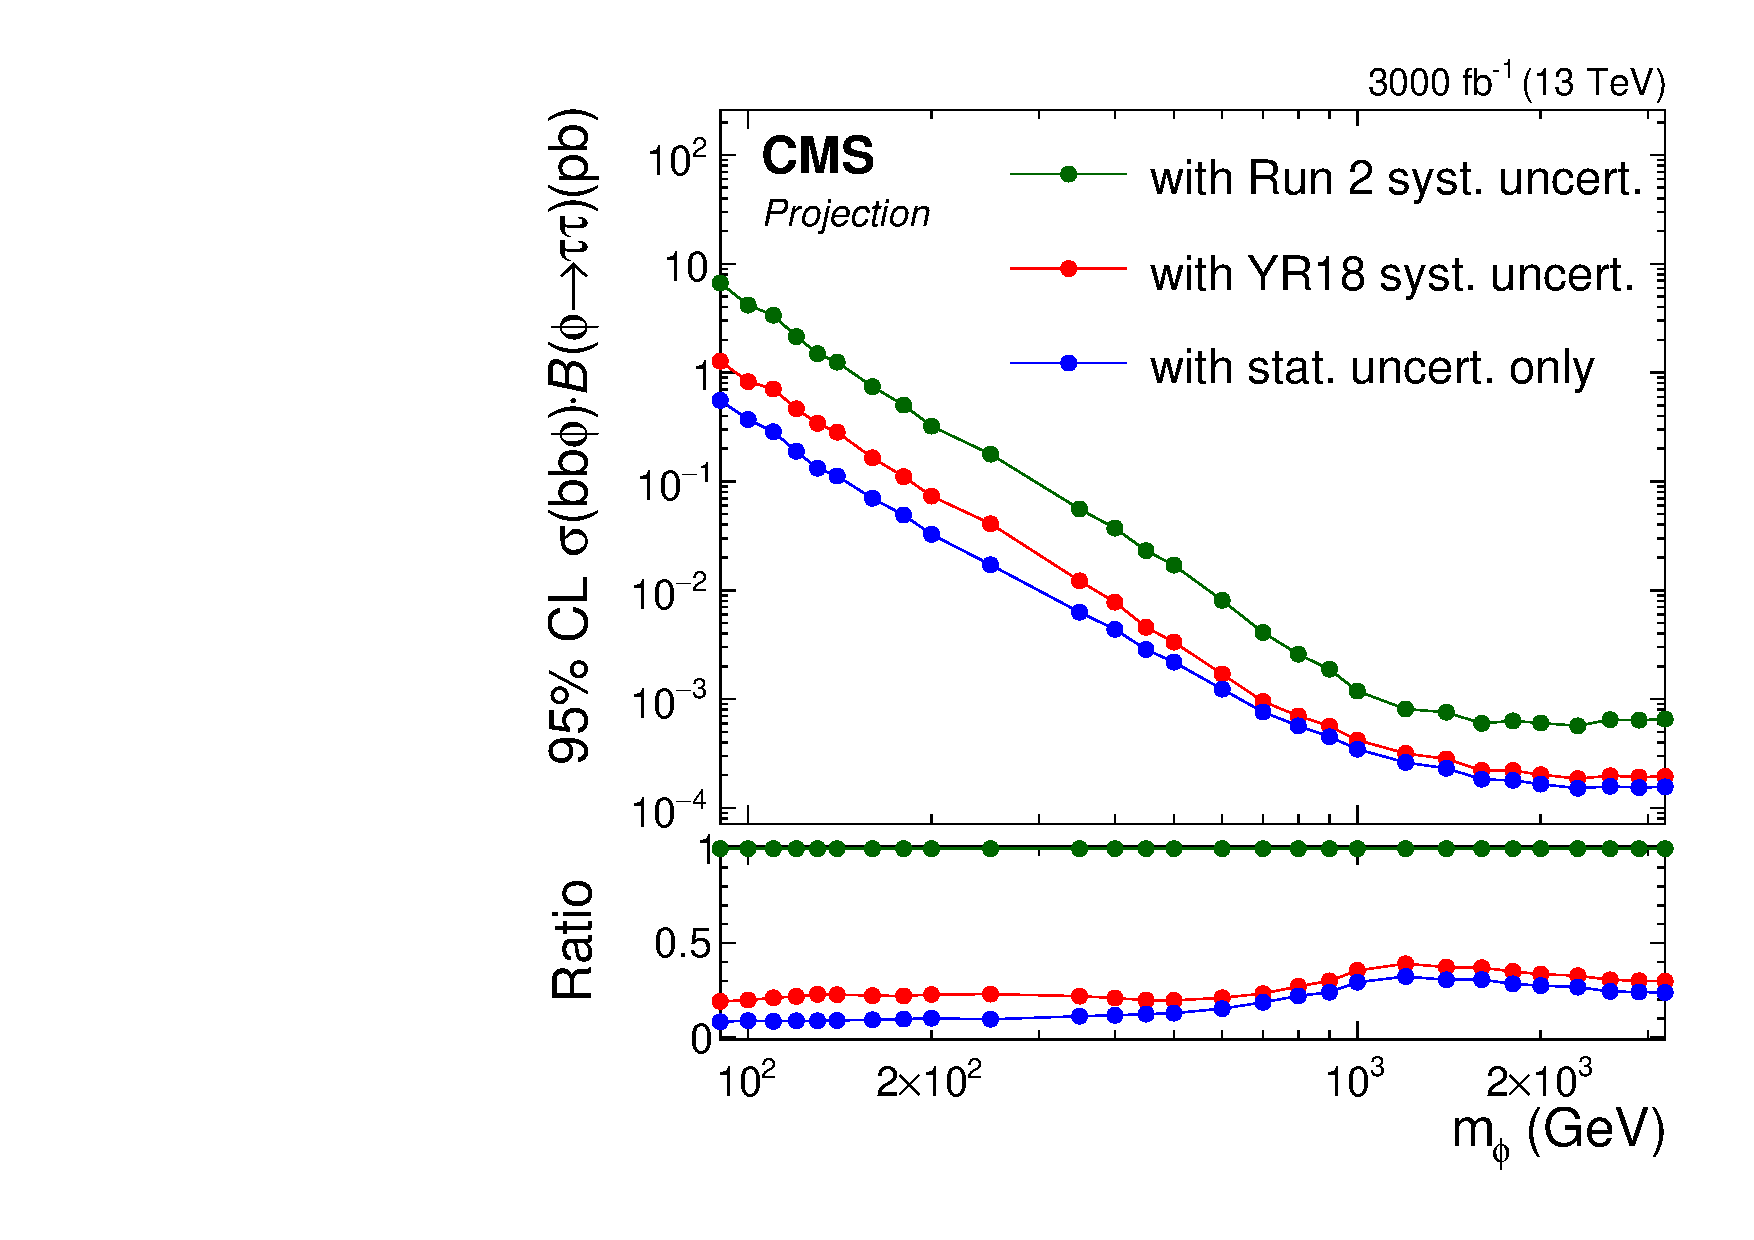
\includegraphics[width=0.45\textwidth]{\main/section9/plots/3000fb_bbH_pas.pdf}}
\end{center}
\caption{Projection of expected model-independent limits based on 2016 data~\cite{HIG-17-020} for ggH and bbH production with subsequent \htt decays, comparing different 
scenarios for systematic uncertainties for an integrated luminosity of 3000\fbinv.}
\label{fig:model_indep2}
\end{figure}
